\setlength{\baselineskip}{20pt}
\chapter{引言}
\label{cha:intro}

\makeatletter
\renewcommand{\cleardoublepage}{\relax
  \clearpage
  \if@twoside \ifodd\c@page\relax\else
  \thispagestyle{empty}%
  \tikz[remember picture, overlay] \node  at (current page.center)
    {\large (本页留空)};\newpage\fi\fi}
\makeatother

物畅其流则百业兴,我国正在加速构建以国内大循环为主体,
国内国际双循环相互促进的新发展格局,
打造安全可靠、高效便捷的现代物流网络系统迫在眉睫。
其中,物流网络基础设施节点的科学布局、稳定运行是制约物流网络可靠性的关键要素。
尤其近年来,
物流网络面临愈加频繁的自然灾害、公共卫生事件、复杂多变的国际经济政治形势等突发风险。
因此,如何在物流网络规划阶段就考虑节点失效风险,
高效计算并设计出科学合理、安全可靠的物流网络,
是我国物流业降本增效、抢占``双循环''机遇制高点的一个重要抓手。

\section{研究背景和意义} 
\label{sec:研究背景和意义}

\subsection{研究背景} 
\label{subsec:研究背景}

现代物流是经济发展的``经脉'',连接着生产与消费的全部流程\cite{唐仁敏},
将运输、仓储、包装、配送、装卸搬运、流通加工、信息处理等服务功能高度集成,
是延伸产业链、提升价值链、打造供应链的重要支撑,
是促进国民经济循环畅通的重要抓手\cite{王微}。
在国务院《``十四五''现代物流发展规划》宏伟蓝图的指引下,
我国社会物流效率逐渐稳固提升,市场环境不断向好发展。
近五年来,我国物流经受住了多重压力,
实现了行业稳步增长。
2018年至2022年,我国物流社会总额从283.1万亿元增长至347.6万亿元,
复合年均增长率4.2\% ,
物流业总收入从10.1万亿元增长至12.7万亿元,
复合年均增长率4.7\% % 注意这里不能有标点
\footnotemark。\footnotetext{数据来源:中国物流与采购联合会。}

随着行业的快速发展,
不断增加的物质资源、信息资源和社会生产活动将物流节点连接成一个复杂且精密的网络。
然而,网络中的节点受到诸多自然因素和人为因素的影响从而面临失效风险,
例如2012年北京特大暴雨和2016年1号台风``尼伯特''等自然因素;
2015年天津滨海新区爆炸事件和上海浦东申通三林分公司的罢工事件等人为因素,
直接导致当地部分基础设施节点和线路失效;
2020年新型冠状病毒肺炎疫情爆发,运力资源短缺、运输网络阻隔、
运营安全欠缺等挑战蜂拥而至,
``九省通衢''的武汉节点及关联网络失效,
物流体系受到巨大影响,
且由于针对节点失效风险的物流网络规划较少,
导致物流网络不同程度受损,区域物流网络几近瘫痪,
同时也对国民经济中诸多行业造成雪崩式影响。
因此,在节点选址布局设计时就考虑可能存在的失效风险,
或针对既有网络布局寻求优化方案,从空间布局上适度安排合理的备用节点。
一旦当前常用节点失效,则由其备用节点提供物流服务,
以减少成本、时间上的损失,提高整个物流网络的可靠性。

此外,即便在信息化高度发达的当今社会,
物流节点失效也常常伴随电力设施损毁、基础通信设施破坏,
导致信息传递不及时甚至中断;
亦或者客户已知节点损坏,
但不确定因素导致客户不清楚节点何时可以恢复服务。
此时,
客户不能准确判断节点能否或何时提供服务,
处于一种``不完全信息''的状态。
在不完全信息的状态下,
客户通常会采取一种试错策略,
以寻求可能存在的服务。
在现实生活的各个行业中,这种试错策略很普遍:
对于零售企业(商场、零售店等)或是基础服务设施(电动汽车充电桩、停车场、ATM机等)来说,
在客户到达这类设施之前,并不能准确知道自己是否可以被该设施服务,
因此决定先前往试一试运气,如果不能被服务则前往下一个设施。
在物流行业中,除了末端零售节点以外,
客户采用试错策略访问中转节点的场景也有很多:
例如,早年的``双十一购物节'',快递爆仓时有发生,
若大量快递滞留在某个中转中心来不及处理,则可能被转运至其他中转中心以分散压力。
另一个近期的案例是2021年5月下旬,
作为世界上第三大港口的深圳盐田港因港区工人确诊新冠肺炎导致严重的货物积压,
不得不暂停了五天的集装箱入闸业务,
恢复后也只能在短时间内接受船舶预计到港日期前三天内的出口重柜\cite{盐田港}。
在暂停业务的期间,
一部分集装箱选择绕过该港口尝试从其他港口出港,
但成本有会有不同程度的提升。

在不完全信息场景下,
虽然只有一个节点为客户的单次需求提供服务,
但每个客户可能有多个节点为其长期提供备用服务。
客户的试错策略可能使得客户在寻求服务时逐个访问多个节点,
使得节点之间产生了额外联系。
这些节点距离客户的远近不同。
相应地,客户寻求服务时也以总期望成本最小的顺序逐个尝试。
然而,一般的经典选址模型(例如P-中心、P-中值、集合覆盖模型等)
假设设施建设后能持续为客户提供服务,
并未预留一个使客户在设施失效后能够及时获得服务的备用方案或容错方案。
在本世纪初的选址理论发展过程中,
可靠固定成本选址(Reliable Fixed-charge Location, RFL)
理论被提出\cite{Snyder2005},
旨在解决上述经典理论中未考虑到的失效因素。
RFL模型考虑了设施失效的情况,即假定每个设施在建成后都存在损坏的概率。
为了在设施损坏时尽可能降低损失,
在规划初期,RFL模型为每个客户指派了一个常用设施之外,还指派了多个备用设施。
通过``一个常用设施,多个备用设施''的策略,
RFL模型降低了常用设施损坏时,因临时决策产生的高昂成本。
本文的第\ref{cha:review}章针对RFL模型的发展现状和理论背景展开了详细的叙述。

针对现实存在的问题和需求,
基于RFL选址理论,
本文研究了考虑节点失效风险的物流网络选址问题,
目的是以一种预先规划的主动强化策略提升物流网络的韧性。
其中,可靠性是指在系统内部某些部分失灵的情况下,
整个系统仍能良好运行的能力\cite{BermanReliability};
不完全信息是指客户对节点的状态没有完全地了解\cite{BermanIncompleteInformation};
试错策略是指客户在常用节点失效后,逐个访问备用节点的过程。
由于在节点阻塞的状态(例如,拥堵、爆仓等)被视为失效状态,
本文在模型的考虑因素中主动忽略了设施的容量限制。
因此,本文研究的模型是可靠无容量固定费用选址问题
(Reliable Uncapacitated Fixed-charge Location, RUFL)的相关拓展和应用,
其原始理论为无容量固定费用选址问题
(Uncapacitated Fixed-charge Location, UFL)\cite{Snyder2005},
同时也是网络和离散选址问题的一个分支\cite{Daskin书}。
另外,
从上述介绍可知本文研究的不完全信息场景适用于设施端提供服务的节点,
例如末端零售、中转节点、港口、仓库等。
区别于狭义的``消费者''的概念,
本文考虑的客户是一个广义的角色,是指接受节点服务的个人或组织。
例如,对于快递的中转中心来说,狭义的客户是指快递的收件人,
但本文考虑的广义客户是物流公司自身,
因为其接受了中转中心的服务。
最后,值得一提的是本文讨论的问题并不针对于某种特殊的物流节点类型,
而是提出了一个普适的、与物流节点相关的可靠选址理论,
第\ref{subsec:研究意义}节阐明了研究该理论的现实意义和理论意义。

\subsection{研究意义}  % 1.1.2 
\label{subsec:研究意义}
上述内容中提到,物流节点是物流网络中的重要组成,
承担了物流基础活动中除运输之外的大部分功能,
如分拣、仓储、包装、搬运、流通加工等\cite{董鹏}。
研究物流节点的可靠选址问题,有利于构建一个具有韧性的、
可靠的现代物流网络。本文的研究意义可分为现实意义和理论意义:

从现实意义出发,由于设施的建设成本较高,且建设后将长期提供服务,
因而选址问题成为企业长期的战略问题。
错误的选址决策会导致运营成本增加和企业竞争力下降\cite{Daskin书}。
在物流网络拓扑结构设计之初,考虑物流节点失效和不完全信息场景,
将降低运营过程中由于节点失效导致的高昂损失,
提升节点失效时物流网络的运营效率,为客户提供更加优质的物流服务。

从理论意义出发,本文研究的物流节点选址问题,丰富了相关选址理论,
是RUFL理论的进一步深化和实际应用。
本文采用了数学优化方法对现实问题进行抽象并建模,
虽然所求解的模型的最优性是数学意义上的,
但是建模的过程(分析目标函数和约束,收集并整理数据)
也为改进选址决策提供了参考和依据。
此外,求解模型的过程,丰富了相关算法理论研究,
是拉格朗日松弛算法求解大规模整数规划问题的具体实践。

\subsection{研究创新点} % 1.2
\label{subsec:创新点}
本文研究的问题是RFL理论的进一步拓展和应用,
从物流节点的角度出发,考虑了节点可能失效的情况与应对失效的措施;
从广义客户的角度出发,考虑了信息的不完全性以及客户接受服务的试错过程;
刻画了客户的行为,并计算了期望成本;
为了求解该问题的大规模实例,定制了优化算法。
综上,本文的创新点集中体现在模型创新与算法创新两个方面,
具体如下:
\begin{enumerate}[label=(\arabic*),leftmargin=0pt,itemindent=3.5\ccwd,nosep]
  \item 考虑了物流节点的失效风险。
  在传统物流节点选址问题中,通常认为节点在建成后可以持续为客户提供服务,
  然而在现实中,节点所处环境中的风险可能导致节点失效。
  本文将节点的失效概率纳入模型中,
  这使得模型更加贴近现实,
  优化的结果也更具现实意义。

  \item 描述了客户在节点失效时尝试获取服务的试错策略,
  引入了客户在不能接受服务时产生的试错过程,
  这种试错过程是应对设施失效、强化网络可靠性的方法之一,
  但很少出现在选址理论的研究中。
  将客户试错过程与设施失效相结合,
  并体现在模型构建中,
  是考虑节点失效风险的物流网络选址模型的创新之处。

  \item 设计了基于迭代局部搜索改进的拉格朗日松弛算法。
  由于研究的问题是非确定性多项式难
  (Non-deterministic Polynomial Hard, NP-hard)类型,
  问题的规模随节点数量的增加指数级增长。
  本文为该问题定制的混合优化算法
  可以有效求解大规模的算例。
  该算法能够得到一个高质量下界,
  并通过多种精确和启发式方法保证了上界的质量。
  算法精心设计的拉格朗日乘子初始化及更新规则
  可使得上下界快速收敛并证明解的优劣。
\end{enumerate}

\section{研究路线} % 1.2
\label{sec:研究路线}
针对物流节点可能失效的情况,
考虑到节点失效同时信息的不完全特性以及选址决策的特点,
本文对考虑节点失效风险的物流网络选址问题进行研究。
本文的技术路线如图\ref{fig:技术路线}所示,
全文共分为6个章节,每章的内容如下:

\begin{figure}[t] 
  \setlength{\belowcaptionskip}{-0.5cm} 
  \centering
  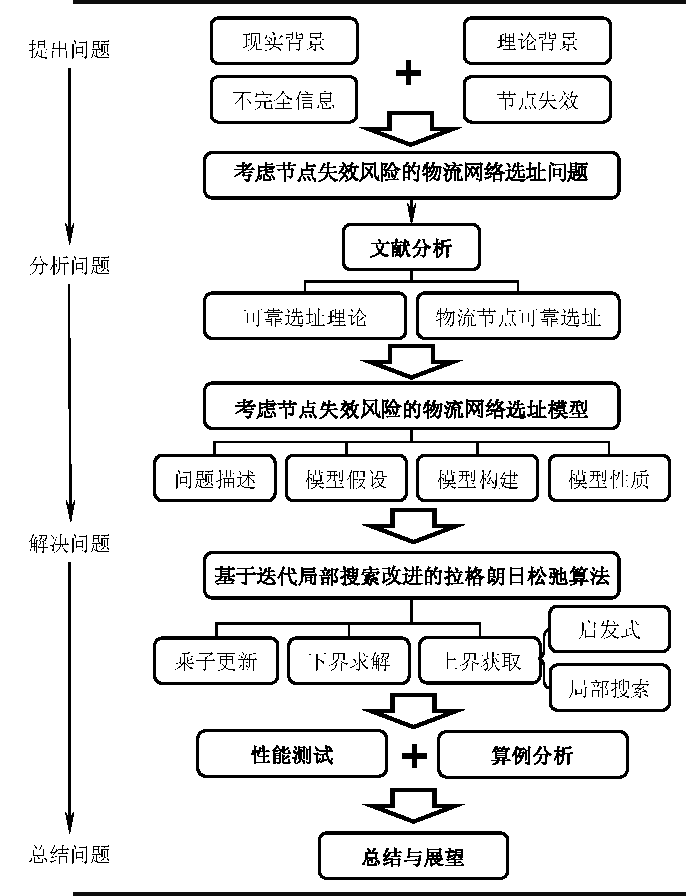
\includegraphics[height=0.7\textheight]{figures/route_.pdf}
  \caption{技术路线 \\Fig~\ref{fig:技术路线}~Technical Route}
  \label{fig:技术路线}
\end{figure}

第\ref{cha:intro}章介绍了本文的研究背景,
从繁荣发展的物流行业背后仍存在节点失效的现象出发,
引出本文的研究主题。
结合研究背景,从理论和现实两个方面明确了本文的研究意义;
分别从模型与算法两个角度阐明本文的创新性;
确定了本文的研究路线和文章结构安排。

第\ref{cha:review}章首先回顾并总结了可靠选址理论的发展过程,
着重总结了一系列建模考虑的因素和求解模型的算法,
指出了研究的薄弱之处和未来可能的研究方向。
然后简要概述了可靠选址理论在物流选址问题中的应用,
特别是相关考虑因素和解决方案。

第\ref{cha:model}章为考虑节点失效风险的物流网络选址问题构建了数学模型,
并证明了该问题的NP-hard属性。
由于该模型属于混合整数规划(Mixed Integer Programming, MIP)类型,
且带有二次约束和二次目标项,
第\ref{cha:model}章中应用了线性化技术消除模型的二次成分。
此外,模型性质分析中还讨论了一个子问题,
本文称为试错序列问题,该问题是基本最短路问题更为广泛的形式之一。

第\ref{cha:LR算法}章开发了基于迭代局部搜索改进的拉格朗日松弛算法,
从一个一般问题出发推导算法的基本原理,
并开发了一系列求解上界、下界的精确方法和启发式方法,
详细阐述了算法的控制流程。

第\ref{cha:算法性能章}章采用经典测试数据集验证了算法的性能和有效性,
对比了算法与商业求解器之间的性能差异,
分析了算法中重要算子的性能。
并对算例数据中的重要参数
进行了参数灵敏度分析,从分析结果中给出管理学启示。

第\ref{cha:summary}章总结了全文,指出本文研究工作的不足和待完善之处,
并展望了该问题未来的研究方向和研究内容。


\section{本章小结} % 1.2
\label{sec:引言小结}
本章确定了考虑节点失效风险的物流网络选址问题的研究背景,
通过现实案例介绍了物流节点所面临的失效风险以及客户的试错策略。
此外,本章介绍了研究的理论意义和现实意义以及模型和算法的创新性。
最后,确定了本文的研究思路和文章架构。
在讨论的过程中,明确了本文研究的问题基于可靠选址问题。
因此,第\ref{cha:review}章回顾了可靠选址问题相关的研究,
特别是与物流节点选址相关的文献。
